\documentclass{article}

% content/resources/templates/preamble.tex
\usepackage[margin=0.6in]{geometry}
\author{Milav Dabgar}
\usepackage{amsmath,amssymb,amsthm}
\usepackage{booktabs}
\usepackage{multirow}
\usepackage{xcolor}
\usepackage{tcolorbox}
\tcbuselibrary{breakable,skins}
\usepackage[colorlinks=true,linkcolor=blue]{hyperref}
\usepackage{titlesec}
\usepackage{enumitem}
\usepackage{tikz}
\usepackage{pgfplots}
\usepackage{circuitikz}
\usepackage[version=4]{mhchem}
\usepackage{longtable}
\usepackage{array}
\usepackage{float}
\usepackage{caption}
\usepackage{listings}

\lstset{
  basicstyle=\small\ttfamily,
  breaklines=true,
  breakatwhitespace=false,
  postbreak=\mbox{\textcolor{red}{$\hookrightarrow$}\space},
  float=false,
  numbers=left,
  numberstyle=\tiny\color{gray},
  numbersep=10pt,
  xleftmargin=2em,
  keywordstyle=\color{blue},
  commentstyle=\color{green!60!black},
  stringstyle=\color{purple},
  backgroundcolor=\color{gray!5},
  showstringspaces=false,
  tabsize=2,
  captionpos=b,
  keepspaces=true,
  columns=flexible
}

\pgfplotsset{compat=1.18}
\usetikzlibrary{shapes,arrows,positioning,calc,patterns,decorations.pathmorphing,decorations.markings,arrows.meta}

% Color scheme
\definecolor{headcolor}{RGB}{0,102,204}
\definecolor{keycolor}{RGB}{220,20,60}
\definecolor{solutioncolor}{RGB}{34,139,34}
\definecolor{mnemoniccolor}{RGB}{148,0,211}
\definecolor{codecolor}{RGB}{0,0,100}

% Spacing
\setlength{\parskip}{3pt}
\setlist[itemize]{nosep}
\setlist[enumerate]{nosep}

% Title formatting
\titleformat{\section}{\Large\bfseries\color{headcolor}}{\thesection}{1em}{}
\titleformat{\subsection}{\large\bfseries\color{headcolor}}{\thesubsection}{1em}{}

% Pandoc tightlist compatibility
\providecommand{\tightlist}{%
  \setlength{\itemsep}{0pt}\setlength{\parskip}{0pt}}

% Pandoc longtable compatibility
\newcounter{none}
\def\thenone{}


% content/resources/templates/english-boxes.tex

% Custom environments
\newtcolorbox{solutionbox}{
 breakable,
 enhanced,
 colback=solutioncolor!5!white,
 colframe=solutioncolor!75!black,
 fonttitle=\bfseries,
 title=Solution
}

\newtcolorbox{solutionboxnobreak}{
 colback=solutioncolor!5!white,
 colframe=solutioncolor!75!black,
 fonttitle=\bfseries,
 title=Solution
}

\newtcolorbox{keyformula}{
 breakable,
 enhanced,
 colback=keycolor!5!white,
 colframe=keycolor!75!black,
 fonttitle=\bfseries,
 title=Key Formula
}

\newtcolorbox{mnemonicboxenv}{
 breakable,
 enhanced,
 colback=mnemoniccolor!5!white,
 colframe=mnemoniccolor!75!black,
 fonttitle=\bfseries,
 title=Mnemonic
}

\newcommand{\mnemonicbox}[1]{%
  \begin{mnemonicboxenv}
    #1
  \end{mnemonicboxenv}
}


% Custom commands for GTU solutions
% This file defines semantic commands for consistent formatting

% Question command with automatic formatting
\newcommand{\question}[2]{%
  \section*{Question #1}%
  \textbf{#2}%
}

% OR question variant
\newcommand{\questionor}[2]{%
  \section*{Question #1 OR}%
  \textbf{#2}%
}

% Proper table environment with caption
\newenvironment{answertable}[1]{%
  \begin{table}[htbp]
  \centering
  \caption{#1}
}{%
  \end{table}
}

% Proper figure environment for diagrams
\newenvironment{answerdiagram}[1]{%
  \begin{figure}[htbp]
  \centering
  \caption{#1}
}{%
  \end{figure}
}

% Semantic markup for key terms
\newcommand{\keyword}[1]{\textbf{#1}}
\newcommand{\code}[1]{\texttt{#1}}
\newcommand{\classname}[1]{\texttt{#1}}
\newcommand{\methodname}[1]{\texttt{#1}}

% Proper quotation marks
\newcommand{\mnemonic}[1]{``#1''}

\usetikzlibrary{fit}

\title{Linux Operating System (4331602) - Winter 2023 Solution}
\date{January 16, 2024}

\begin{document}
\maketitle

\questionmarks{1(a)}{3}{Draw the architecture of Linux and explain various layers in brief.}

\begin{solutionbox}
\textbf{Answer}:

\textbf{Linux Architecture:}

\begin{center}
\begin{tikzpicture}[node distance=1.5cm]
    \node [gtu block, minimum width=8cm] (user) {User Applications};
    \node [gtu block, minimum width=8cm, below=0.5cm of user] (shell) {System Call Interface / Shell};
    \node [gtu block, minimum width=8cm, minimum height=2cm, below=0.5cm of shell] (kernel) {Kernel \\ (Process, Memory, File, Network Management)};
    \node [gtu block, minimum width=8cm, below=0.5cm of kernel] (drivers) {Device Drivers};
    \node [gtu block, minimum width=8cm, below=0.5cm of drivers] (hw) {Hardware};

    \draw [gtu arrow] (user) -- (shell);
    \draw [gtu arrow] (shell) -- (kernel);
    \draw [gtu arrow] (kernel) -- (drivers);
    \draw [gtu arrow] (drivers) -- (hw);
\end{tikzpicture}
\captionof{figure}{Linux Architecture}
\end{center}

\textbf{Layers:}
\begin{itemize}
    \item \keyword{User Space}: Contains user applications and system utilities.
    \item \keyword{System Call Interface}: Provides interface between user programs and kernel.
    \item \keyword{Kernel Space}: Core operating system responsible for resource management.
    \item \keyword{Hardware}: Physical components of the computer system.
\end{itemize}
\end{solutionbox}

\begin{mnemonicbox}
\mnemonic{USKDH - Users System Kernel Drives Hardware}
\end{mnemonicbox}

\questionmarks{1(b)}{4}{What is a race condition? Explain with a suitable example.}

\begin{solutionbox}
\textbf{Answer}:

\begin{center}
\captionof{table}{Race Condition}
\begin{tabulary}{\linewidth}{|L|L|}
\hline
\textbf{Aspect} & \textbf{Description} \\ \hline
Definition & Situation where multiple processes access shared resources simultaneously \\ \hline
Problem & Unpredictable results depending on execution order \\ \hline
Example & Bank account balance update by simultaneous transactions \\ \hline
\end{tabulary}
\end{center}

\textbf{Example Scenario:}
\begin{enumerate}
    \item \keyword{Process A}: Reads balance = 1000, adds 100 (ready to write 1100).
    \item \keyword{Process B}: Reads balance = 1000 (before A writes), subtracts 50 (ready to write 950).
    \item \keyword{Result}: Final balance could be 1100 or 950, instead of correct 1050, depending on who writes last.
\end{enumerate}
\end{solutionbox}

\begin{mnemonicbox}
\mnemonic{RRRR - Race Results Random Resources}
\end{mnemonicbox}

\questionmarks{1(c)}{7}{List different types of Operating systems. Explain the working of multiprogramming operating systems with a suitable example.}

\begin{solutionbox}
\textbf{Answer}:

\textbf{Types of Operating Systems:}
\begin{center}
\captionof{table}{Types of Operating Systems}
\begin{tabulary}{\linewidth}{|L|L|}
\hline
\textbf{Type} & \textbf{Characteristics} \\ \hline
Batch & Jobs processed in groups without user interaction \\ \hline
Time-sharing & Multiple users share system simultaneously \\ \hline
Real-time & Strict time constraints for operations \\ \hline
Distributed & Computations distributed among networked processors \\ \hline
Multiprogramming & Multiple programs kept in memory for CPU utilization \\ \hline
\end{tabulary}
\end{center}

\textbf{Multiprogramming Working:}
\begin{itemize}
    \item \keyword{Memory Management}: Multiple jobs are kept in main memory simultaneously.
    \item \keyword{CPU Utilization}: When one job waits for I/O, CPU switches to another job.
    \item \keyword{Context Switching}: OS saves state of current job and loads state of next job.
\end{itemize}

\textbf{Example}: A user running a web browser, music player, and word processor simultaneously. While browser waits for network data, CPU executes music player instructions.
\end{solutionbox}

\begin{mnemonicbox}
\mnemonic{MPMP - Multiple Programs Maximize Performance}
\end{mnemonicbox}

\questionmarks{1(c) OR}{7}{List different types of Operating systems. Explain the Batch operating systems in detail.}

\begin{solutionbox}
\textbf{Answer}:

\textbf{Types of Operating Systems:}
(Same as above table)

\textbf{Batch Operating System:}
\begin{itemize}
    \item \keyword{Job Collection}: Users submit jobs (program + data + control info) offline.
    \item \keyword{Batching}: Operator groups similar jobs into batches to speed up processing.
    \item \keyword{Sequential Execution}: CPU executes jobs in a batch one after another.
    \item \keyword{No Interaction}: User cannot interact with the job during execution.
\end{itemize}

\textbf{Advantages and Disadvantages:}
\begin{itemize}
    \item \textbf{Pros}: High CPU utilization for similar jobs, simple to manage.
    \item \textbf{Cons}: Long turnaround time, difficult to debug, no real-time capability.
\end{itemize}
\end{solutionbox}

\begin{mnemonicbox}
\mnemonic{BBBB - Batch Brings Better Business}
\end{mnemonicbox}

\questionmarks{2(a)}{3}{Draw and explain the Process life cycle.}

\begin{solutionbox}
\textbf{Answer}:

\begin{center}
\begin{tikzpicture}[node distance=2cm, auto]
    \node [gtu state] (new) {New};
    \node [gtu state, right=of new] (ready) {Ready};
    \node [gtu state, right=of ready] (running) {Running};
    \node [gtu state, right=of running] (term) {Terminated};
    \node [gtu state, below=of ready] (wait) {Waiting};

    \path [gtu arrow] (new) -- node {Admit} (ready);
    \path [gtu arrow] (ready) -- node {Dispatch} (running);
    \path [gtu arrow] (running) -- node {Exit} (term);
    \path [gtu arrow] (running) edge [bend right] node [above] {Interrupt} (ready);
    \path [gtu arrow] (running) -- node {I/O Wait} (wait);
    \path [gtu arrow] (wait) -- node {I/O Complete} (ready);
\end{tikzpicture}
\captionof{figure}{Process State Diagram}
\end{center}

\textbf{States:}
\begin{itemize}
    \item \keyword{New}: Process is being created.
    \item \keyword{Ready}: Process is waiting to be assigned to a processor.
    \item \keyword{Running}: Instructions are being executed.
    \item \keyword{Waiting}: Process is waiting for some event (I/O).
    \item \keyword{Terminated}: Process has finished execution.
\end{itemize}
\end{solutionbox}

\begin{mnemonicbox}
\mnemonic{NRWRT - New Ready Waiting Running Terminated}
\end{mnemonicbox}

\questionmarks{2(b)}{4}{Define deadlock and discuss necessary conditions for a deadlock to occur.}

\begin{solutionbox}
\textbf{Answer}:

\textbf{Deadlock}: A situation where a set of processes are blocked because each process is holding a resource and waiting for another resource acquired by some other process.

\textbf{Coffman Conditions (All must hold):}
\begin{enumerate}
    \item \keyword{Mutual Exclusion}: At least one resource must be held in a non-shareable mode.
    \item \keyword{Hold and Wait}: A process holds a resource while waiting for another.
    \item \keyword{No Preemption}: Resources cannot be forcibly taken from a process.
    \item \keyword{Circular Wait}: A set of processes $\{P0, P1, \dots, Pn\}$ exists such that $P0$ waits for $P1$, $P1$ waists for $P2$, \dots, $Pn$ waits for $P0$.
\end{enumerate}
\end{solutionbox}

\begin{mnemonicbox}
\mnemonic{MHNC - My Hold Never Circles}
\end{mnemonicbox}

\questionmarks{2(c)}{7}{Describe the Round Robin algorithm. Calculate the average waiting time \& average turn-around time along with Gantt chart for the given data. Consider context switch = 01 ms and quantum time = 05 ms.}

\begin{solutionbox}
\textbf{Answer}:

\textbf{Round Robin Algorithm:}
Preemptive scheduling where each process gets a small unit of CPU time (time quantum).

\textbf{Given Data:} Context Switch = 1ms, Quantum = 5ms.

\textbf{Processes:}
\begin{center}
\begin{tabular}{|c|c|c|}
\hline
Process & Arrival & Burst \\ \hline
P1 & 0 & 12 \\ \hline
P2 & 3 & 4 \\ \hline
P3 & 2 & 15 \\ \hline
P4 & 5 & 5 \\ \hline
\end{tabular}
\end{center}

\textbf{Gantt Chart:}
\begin{center}
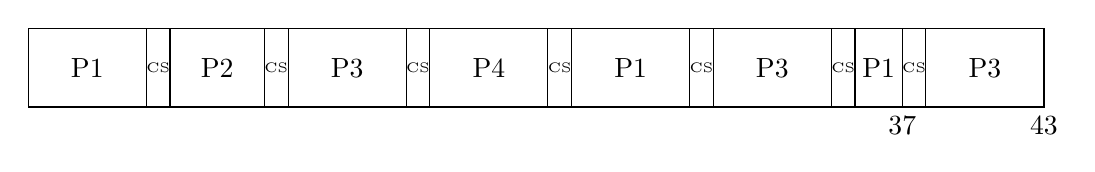
\begin{tikzpicture}[x=0.3cm, y=1cm]
    \draw (0,0) rectangle (5,1) node[midway] {P1};
    \draw (5,0) rectangle (6,1) node[midway, font=\tiny] {CS};
    \draw (6,0) rectangle (10,1) node[midway] {P2};
    \draw (10,0) rectangle (11,1) node[midway, font=\tiny] {CS};
    \draw (11,0) rectangle (16,1) node[midway] {P3};
    \draw (16,0) rectangle (17,1) node[midway, font=\tiny] {CS};
    \draw (17,0) rectangle (22,1) node[midway] {P4};
    \draw (22,0) rectangle (23,1) node[midway, font=\tiny] {CS};
    \draw (23,0) rectangle (28,1) node[midway] {P1};
    \draw (28,0) rectangle (29,1) node[midway, font=\tiny] {CS};
    \draw (29,0) rectangle (34,1) node[midway] {P3};
    \draw (34,0) rectangle (35,1) node[midway, font=\tiny] {CS};
    \draw (35,0) rectangle (37,1) node[midway] {P1}; \node[below] at (37,0) {37};
    \draw (37,0) rectangle (38,1) node[midway, font=\tiny] {CS};
    \draw (38,0) rectangle (43,1) node[midway] {P3}; \node[below] at (43,0) {43};
\end{tikzpicture}
\captionof{figure}{Gantt Chart (RR)}
\end{center}
\textit{Note: Calculated based on problem statement logic. P1(5) $\to$ P2(4) $\to$ P3(5) $\to$ P4(5) $\to$ P1(5) $\to$ P3(5) $\to$ P1(2) $\to$ P3(5).}

\textbf{Calculations:}
\begin{center}
\begin{tabulary}{\linewidth}{|L|L|L|L|L|}
\hline
\textbf{Process} & \textbf{Completion} & \textbf{Turnaround} & \textbf{Waiting} \\ \hline
P1 & 37 & 37 - 0 = 37 & 37 - 12 = 25 \\ \hline
P2 & 10 & 10 - 3 = 7 & 7 - 4 = 3 \\ \hline
P3 & 43 & 43 - 2 = 41 & 41 - 15 = 26 \\ \hline
P4 & 22 & 22 - 5 = 17 & 17 - 5 = 12 \\ \hline
\end{tabulary}
\end{center}

\textbf{Average Waiting Time} = $(25 + 3 + 26 + 12)/4 = 16.5$ ms
\textbf{Average Turnaround Time} = $(37 + 7 + 41 + 17)/4 = 25.5$ ms
\end{solutionbox}

\begin{mnemonicbox}
\mnemonic{RRRR - Round Robin Rotates Regularly}
\end{mnemonicbox}

\questionmarks{2(a) OR}{3}{Differentiate: CPU bound process v/s I/O bound process.}

\begin{solutionbox}
\textbf{Answer}:

\begin{center}
\captionof{table}{CPU vs I/O Bound}
\begin{tabulary}{\linewidth}{|L|L|L|}
\hline
\textbf{Aspect} & \textbf{CPU Bound} & \textbf{I/O Bound} \\ \hline
Activity & High CPU computations & Frequent I/O operations \\ \hline
Burst Time & Long CPU bursts & Short CPU bursts \\ \hline
Wait States & Less frequent & Frequent waiting for I/O \\ \hline
Examples & Scientific calculation & Data processing, File copy \\ \hline
\end{tabulary}
\end{center}
\end{solutionbox}

\begin{mnemonicbox}
\mnemonic{CIC - CPU Computes I/O Interacts}
\end{mnemonicbox}

\questionmarks{2(b) OR}{4}{Define Critical Section and discuss the general structure of a critical section solution.}

\begin{solutionbox}
\textbf{Answer}:

\textbf{Critical Section}: Code segment where shared resources (variables, files) are accessed. Only one process should execute in CS at a time.

\textbf{General Structure:}
\begin{lstlisting}[basicstyle=\ttfamily]
do {
    entry section   // Request permission
       critical section
    exit section    // Release permission
       remainder section
} while (true);
\end{lstlisting}

\textbf{Requirements:}
\begin{itemize}
    \item \keyword{Mutual Exclusion}: Only one process in CS.
    \item \keyword{Progress}: If CS is empty, selection of next process cannot be postponed indefinitely.
    \item \keyword{Bounded Waiting}: Waiting time for entry must be limited.
\end{itemize}
\end{solutionbox}

\begin{mnemonicbox}
\mnemonic{ECER - Entry Critical Exit Remainder}
\end{mnemonicbox}

\questionmarks{2(c) OR}{7}{Describe the SJF algorithm. Calculate the average waiting time and average turn-around time along with Gantt chart for the given data.}

\begin{solutionbox}
\textbf{Answer}:

\textbf{Shortest Job First (SJF)}: Non-preemptive algorithm where process with shortest CPU burst is scheduled first.

\textbf{Execution Order}: P1(8), P2(4), P3(9), P4(5).
Order based on arrival and burst:
1. t=0, P1 arrives (8). Runs 0-8.
2. t=8, P2(4), P3(9), P4(5) available. P2 shortest. Runs 8-12.
3. t=12, P4(5), P3(9) avail. P4 shortest. Runs 12-17.
4. t=17, P3(9) runs. Runs 17-26.

\textbf{Gantt Chart (SJF):}
\begin{center}
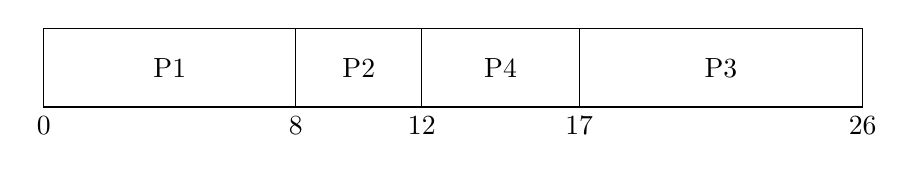
\begin{tikzpicture}[x=0.4cm, y=1cm]
    \draw (0,0) rectangle (8,1) node[midway] {P1};
    \draw (8,0) rectangle (12,1) node[midway] {P2};
    \draw (12,0) rectangle (17,1) node[midway] {P4};
    \draw (17,0) rectangle (26,1) node[midway] {P3};
    
    \node[below] at (0,0) {0};
    \node[below] at (8,0) {8};
    \node[below] at (12,0) {12};
    \node[below] at (17,0) {17};
    \node[below] at (26,0) {26};
\end{tikzpicture}
\captionof{figure}{Gantt Chart (SJF)}
\end{center}

\textbf{Calculations:}
\begin{center}
\begin{tabulary}{\linewidth}{|L|L|L|L|L|L|}
\hline
Process & Arr & Burst & Comp & TAT & Wait \\ \hline
P1 & 0 & 8 & 8 & 8 & 0 \\ \hline
P2 & 3 & 4 & 12 & 9 & 5 \\ \hline
P4 & 6 & 5 & 17 & 11 & 6 \\ \hline
P3 & 5 & 9 & 26 & 21 & 12 \\ \hline
\end{tabulary}
\end{center}

\textbf{Avg Wait} = $(0+5+6+12)/4 = 5.75$ ms
\textbf{Avg TAT} = $(8+9+11+21)/4 = 12.25$ ms
\end{solutionbox}

\begin{mnemonicbox}
\mnemonic{SJSS - Shortest Jobs Start Soon}
\end{mnemonicbox}

\questionmarks{3(a)}{3}{Explain two-level directory structure.}

\begin{solutionbox}
\textbf{Answer}:

\begin{center}
\begin{tikzpicture}[node distance=1.5cm]
    \node [gtu block, minimum width=4cm] (mfd) {Master File Directory};
    \node [gtu block, below left=1cm of mfd] (u1) {User 1 Dir};
    \node [gtu block, below right=1cm of mfd] (u2) {User 2 Dir};
    
    \node [gtu block, below=0.5cm of u1, minimum width=1.5cm] (f1) {File X};
    \node [gtu block, below=0.5cm of u2, minimum width=1.5cm] (f2) {File X};
    
    \draw [gtu arrow] (mfd) -- (u1);
    \draw [gtu arrow] (mfd) -- (u2);
    \draw [gtu arrow] (u1) -- (f1);
    \draw [gtu arrow] (u2) -- (f2);
\end{tikzpicture}
\captionof{figure}{Two-level Directory}
\end{center}

\textbf{Features:}
\begin{itemize}
    \item Separate directory for each user (UFD).
    \item Solves name collision problem (different users can have same filenames).
    \item Provides isolation between users.
\end{itemize}
\end{solutionbox}

\begin{mnemonicbox}
\mnemonic{TTTT - Two Tiers Tackle Troubles}
\end{mnemonicbox}

\questionmarks{3(b)}{4}{Explain the different file operations.}

\begin{solutionbox}
\textbf{Answer}:

\begin{center}
\captionof{table}{File Operations}
\begin{tabulary}{\linewidth}{|L|L|}
\hline
\textbf{Operation} & \textbf{Description} \\ \hline
Create & Allocates space and creates directory entry \\ \hline
Open & Loads file metadata into memory for access \\ \hline
Read & Reads data from current position \\ \hline
Write & Writes data to current position \\ \hline
Delete & Releases space and removes directory entry \\ \hline
Close & Frees internal resources \\ \hline
\end{tabulary}
\end{center}
\end{solutionbox}

\begin{mnemonicbox}
\mnemonic{CORWCD - Create Open Read Write Close Delete}
\end{mnemonicbox}

\questionmarks{3(c)}{7}{List the different file allocation methods and explain contiguous allocation with necessary diagram.}

\begin{solutionbox}
\textbf{Answer}:

\textbf{Methods}: Contiguous, Linked, Indexed.

\textbf{Contiguous Allocation:}
File occupies set of consecutive blocks on disk. Directory entry stores start block and length.

\begin{center}
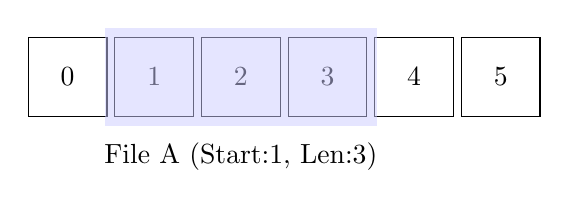
\begin{tikzpicture}[node distance=0cm]
    \foreach \x/\label in {0/0, 1/1, 2/2, 3/3, 4/4, 5/5}
        \node [rectangle, draw, minimum size=1cm] (b\x) at (\x*1.1, 0) {\label};
        
    \node [fit=(b1)(b2)(b3), fill=blue!20, opacity=0.5] {};
    \node [below=0.2cm of b2] {File A (Start:1, Len:3)};
\end{tikzpicture}
\captionof{figure}{Contiguous Allocation}
\end{center}

\textbf{Pros}: Simple (start, length), High performance (fast sequential access).
\textbf{Cons}: External fragmentation, Difficult to grow file.
\end{solutionbox}

\begin{mnemonicbox}
\mnemonic{CCCC - Contiguous Creates Continuous Clusters}
\end{mnemonicbox}

\questionmarks{3(a) OR}{3}{Describe the types of file structures.}

\begin{solutionbox}
\textbf{Answer}:

\begin{itemize}
    \item \keyword{Sequential}: Records stored in order. Simple but slow search.
    \item \keyword{Direct/Random}: Records accessed by key/index. Fast access.
    \item \keyword{Indexed}: Separate index file points to data records.
\end{itemize}
\end{solutionbox}

\begin{mnemonicbox}
\mnemonic{SDI - Sequential Direct Indexed}
\end{mnemonicbox}

\questionmarks{3(b) OR}{4}{Explain the different file attributes.}

\begin{solutionbox}
\textbf{Answer}:

\begin{center}
\captionof{table}{File Attributes}
\begin{tabulary}{\linewidth}{|L|L|}
\hline
\textbf{Attribute} & \textbf{Description} \\ \hline
Name & Human-readable identifier \\ \hline
Type & Format of file (.txt, .exe) \\ \hline
Size & Current file size \\ \hline
Location & Pointer to file location on device \\ \hline
Protection & Access control info (R/W/X) \\ \hline
Time/Date & Info for creation, mod, usage \\ \hline
\end{tabulary}
\end{center}
\end{solutionbox}

\begin{mnemonicbox}
\mnemonic{NTSLPT - Name Type Size Location Permissions Time}
\end{mnemonicbox}

\questionmarks{3(c) OR}{7}{List the different file allocation methods and explain linked allocation with necessary diagram.}

\begin{solutionbox}
\textbf{Answer}:

\textbf{Linked Allocation:}
Files stored in non-contiguous blocks. Each block contains pointer to next block.

\begin{center}
\begin{tikzpicture}[node distance=1.5cm, auto]
    \node [gtu block] (b1) {Block 5 \\ Next: 8};
    \node [gtu block, right=of b1] (b2) {Block 8 \\ Next: 2};
    \node [gtu block, right=of b2] (b3) {Block 2 \\ Next: -1};
    
    \draw [gtu arrow] (b1) -- (b2);
    \draw [gtu arrow] (b2) -- (b3);
\end{tikzpicture}
\captionof{figure}{Linked Allocation}
\end{center}

\textbf{Directory Entry}: Stores pointer to first and last blocks.

\textbf{Pros}: No external fragmentation, easy file growth.
\textbf{Cons}: Slow random access (must traverse chain), pointer overhead.
\end{solutionbox}

\begin{mnemonicbox}
\mnemonic{LLLL - Links Lead Logical Locations}
\end{mnemonicbox}

\questionmarks{4(a)}{3}{Define Program threats and explain its types.}

\begin{solutionbox}
\textbf{Answer}:

\textbf{Program Threats}: Malicious code embedded in program.

\begin{itemize}
    \item \keyword{Trojan Horse}: Appears useful but does damage (steals login).
    \item \keyword{Trap Door}: Secret entry point left by designer.
    \item \keyword{Logic Bomb}: Code that explodes (executes) under specific conditions.
    \item \keyword{Virus}: Code that embeds itself into other programs.
\end{itemize}
\end{solutionbox}

\begin{mnemonicbox}
\mnemonic{TTLV - Trojan Trap Logic Virus}
\end{mnemonicbox}

\questionmarks{4(b)}{4}{Explain System Authentication.}

\begin{solutionbox}
\textbf{Answer}:

\textbf{Authentication}: Verification of user identity.

\textbf{Methods:}
\begin{enumerate}
    \item \keyword{Passwords}: Secret string known to user.
    \item \keyword{Biometrics}: Fingerprint, retina scan, face ID.
    \item \keyword{Smart Cards}: Physical token with embedded chip.
    \item \keyword{Two-Factor}: Combining two methods (e.g., Password + OTP).
\end{enumerate}
\end{solutionbox}

\begin{mnemonicbox}
\mnemonic{PBST - Passwords Biometrics Smartcards Two-factor}
\end{mnemonicbox}

\questionmarks{4(c)}{7}{Explain Access Control List in detail.}

\begin{solutionbox}
\textbf{Answer}:

\textbf{Access Control List (ACL)}: A list associated with each object (file/resource) specifying which domains (users/processes) can access it and how.

\textbf{Structure:}
File X: $(User A, Read), (User B, Read/Write), (Group C, Execute)$

\textbf{Pros}:
\begin{itemize}
    \item Precise control over individual objects.
    \item Easy to revoke permissions for specific users.
\end{itemize}

\textbf{Cons}:
\begin{itemize}
    \item Searching ACL can be slow.
    \item Managing ACLs for many files is complex.
\end{itemize}
\end{solutionbox}

\begin{mnemonicbox}
\mnemonic{ACLU - Access Controls Limit Users}
\end{mnemonicbox}

\questionmarks{4(a) OR}{3}{Define System threats and explain its types.}

\begin{solutionbox}
\textbf{Answer}:

\textbf{System Threats}: Target the environment/OS itself.
\begin{itemize}
    \item \keyword{Worm}: Independent program that spreads through networks consuming resources.
    \item \keyword{Port Scanning}: Detecting open ports to find vulnerabilities.
    \item \keyword{Denial of Service}: Overwhelming system to prevent legitimate use.
\end{itemize}
\end{solutionbox}

\begin{mnemonicbox}
\mnemonic{WPD - Worm Port DoS}
\end{mnemonicbox}

\questionmarks{4(b) OR}{4}{Discuss the needs and goals of protection in OS.}

\begin{solutionbox}
\textbf{Answer}:

\textbf{Needs:}
\begin{itemize}
    \item Prevent malicious misuse of system.
    \item Ensure resources are used fairly.
    \item Protect user data integrity and confidentiality.
\end{itemize}

\textbf{Goals:}
\begin{itemize}
    \item \keyword{Availability}: Resources available to auth users.
    \item \keyword{Integrity}: Data not modified unauthorizedly.
    \item \keyword{Confidentiality}: Data not viewed unauthorizedly.
\end{itemize}
\end{solutionbox}

\begin{mnemonicbox}
\mnemonic{CIA - Confidentiality Integrity Availability}
\end{mnemonicbox}

\questionmarks{4(c) OR}{7}{Discuss various operating system security policies and procedures.}

\begin{solutionbox}
\textbf{Answer}:

\textbf{Policies:}
\begin{itemize}
    \item \keyword{User Policy}: Strong passwords, regular changes.
    \item \keyword{Access Policy}: Least privilege principle.
    \item \keyword{Data Policy}: Encryption of sensitive data.
\end{itemize}

\textbf{Procedures:}
\begin{itemize}
    \item \keyword{Auditing}: Monitoring logs for suspicious activity.
    \item \keyword{Backups}: Regular data backup for recovery.
    \item \keyword{Updates}: Patching OS to fix vulnerabilities.
    \item \keyword{Intrusion Detection}: Systems to detect attacks in real-time.
\end{itemize}
\end{solutionbox}

\begin{mnemonicbox}
\mnemonic{APPI - Access Password Policy Incident}
\end{mnemonicbox}

\questionmarks{5(a)}{3}{Explain the following commands: (i) pwd (ii) cd (iii) comm}

\begin{solutionbox}
\textbf{Answer}:

\begin{center}
\captionof{table}{Commands}
\begin{tabulary}{\linewidth}{|L|L|}
\hline
\textbf{Command} & \textbf{Purpose} \\ \hline
\code{pwd} & Print Working Directory. Shows current path. \\ \hline
\code{cd} & Change Directory. Navigate to different folder. \\ \hline
\code{comm} & Compare two sorted files line by line. \\ \hline
\end{tabulary}
\end{center}
\end{solutionbox}

\begin{mnemonicbox}
\mnemonic{PCC - Pwd Cd Comm}
\end{mnemonicbox}

\questionmarks{5(b)}{4}{Write a shell script to concatenate the contents of two files in a third file.}

\begin{solutionbox}
\begin{lstlisting}[language=bash, caption={Concatenate Files}]
#!/bin/bash
# Script to concatenate two files

echo "Enter first filename:"
read f1
echo "Enter second filename:"
read f2
echo "Enter output filename:"
read f3

if [ -f "$f1" ] && [ -f "$f2" ]; then
    cat "$f1" "$f2" > "$f3"
    echo "Files merged into $f3"
else
    echo "Files not found"
fi
\end{lstlisting}
\end{solutionbox}

\begin{mnemonicbox}
\mnemonic{CCCC - Cat Combines Content Correctly}
\end{mnemonicbox}

\questionmarks{5(c)}{7}{Write a shell script to find the sum of all the individual digits in a given 5 digit number.}

\begin{solutionbox}
\begin{lstlisting}[language=bash, caption={Sum of Digits}]
#!/bin/bash
# Sum of 5 digits

echo "Enter 5 digit number:"
read n

if [ ${#n} -ne 5 ]; then
    echo "Please enter 5 digits"
    exit 1
fi

sum=0
while [ $n -gt 0 ]
do
    rem=$((n % 10))
    sum=$((sum + rem))
    n=$((n / 10))
done

echo "Sum of digits: $sum"
\end{lstlisting}
\end{solutionbox}

\begin{mnemonicbox}
\mnemonic{SSSS - Sum Separates Single Symbols}
\end{mnemonicbox}

\questionmarks{5(a) OR}{3}{Explain the following commands: (i) man (ii) mkdir (iii) grep}

\begin{solutionbox}
\textbf{Answer}:

\begin{center}
\captionof{table}{More Commands}
\begin{tabulary}{\linewidth}{|L|L|}
\hline
\textbf{Cmd} & \textbf{Purpose} \\ \hline
\code{man} & Manual. Displays help/manual for commands. \\ \hline
\code{mkdir} & Make Directory. Creates new folder. \\ \hline
\code{grep} & Global Regular Expression Print. Search text in files. \\ \hline
\end{tabulary}
\end{center}
\end{solutionbox}

\begin{mnemonicbox}
\mnemonic{MMG - Manual Make Grep}
\end{mnemonicbox}

\questionmarks{5(b) OR}{4}{Write a shell script to generate and display Fibonacci series.}

\begin{solutionbox}
\begin{lstlisting}[language=bash, caption={Fibonacci Series}]
#!/bin/bash
# Fibonacci Series

echo "Enter N:"
read n
a=0
b=1

echo -n "$a $b "

for (( i=0; i<n-2; i++ ))
do
    c=$((a + b))
    echo -n "$c "
    a=$b
    b=$c
done
echo ""
\end{lstlisting}
\end{solutionbox}

\begin{mnemonicbox}
\mnemonic{FFFF - Fibonacci Follows Forward Formula}
\end{mnemonicbox}

\questionmarks{5(c) OR}{7}{Write a shell script to determine whether a given string is palindrome.}

\begin{solutionbox}
\begin{lstlisting}[language=bash, caption={Palindrome Check}]
#!/bin/bash
# Palindrome Check

echo "Enter string:"
read str
len=${#str}
rev=""

for (( i=$len-1; i>=0; i-- ))
do
    rev="$rev${str:$i:1}"
done

if [ "$str" == "$rev" ]; then
    echo "Palindrome"
else
    echo "Not Palindrome"
fi
\end{lstlisting}
\end{solutionbox}

\begin{mnemonicbox}
\mnemonic{PPPP - Palindromes Proceed Perfectly Parallel}
\end{mnemonicbox}

\end{document}
